\documentclass[t]{beamer}
\usetheme{hkl}

\title{datasets}
	\author{François Briatte \& Ivaylo Petev}
	\date{Week~\#2}

\begin{document}

  \frame[plain]{
		\titlepage\\[7.25em]
		\begin{columns}[T]
			\column{.50\textwidth}
				\tableofcontents[hideallsubsections]
			\column{.35\textwidth}
				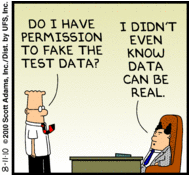
\includegraphics[width=\textwidth]{dilbert-fake-data}
		\end{columns}
	}
	%
	%

  %
  %
  \section{Data sources}
  %
  %

  %
  %
  \subsection{Data philosophy}
  %
  %
  
  \begin{frame}[c, plain]
  
		\href{http://nyti.ms/XSZMFX}%
			{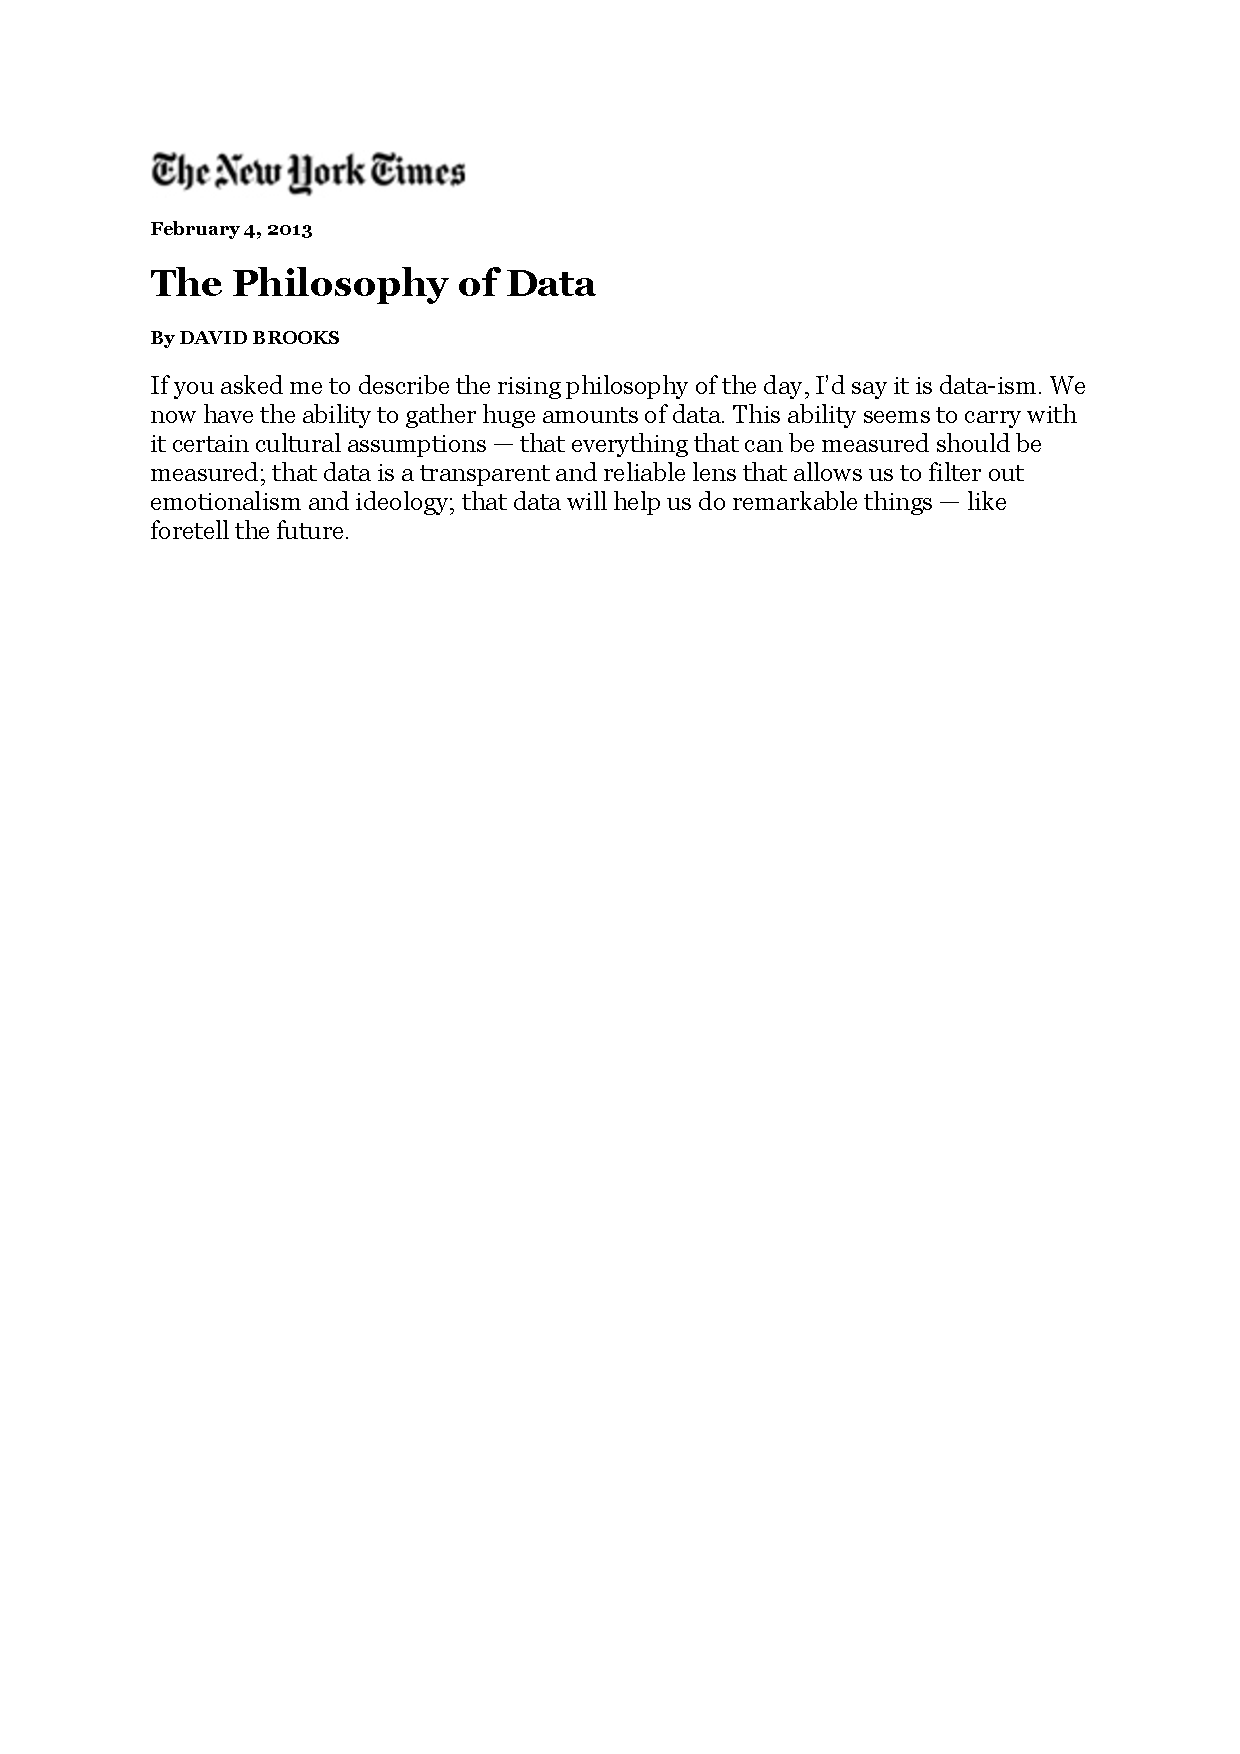
\includegraphics[width=\textwidth]{nyt-philosophy-of-data}}	

  \end{frame}    
	%
	%

  %
  %
  \subsection{Data access}
  %
  %
	
	\begin{frame}[c, plain]

		\begin{center}
			\href{http://www.gapminder.org/}%
  			{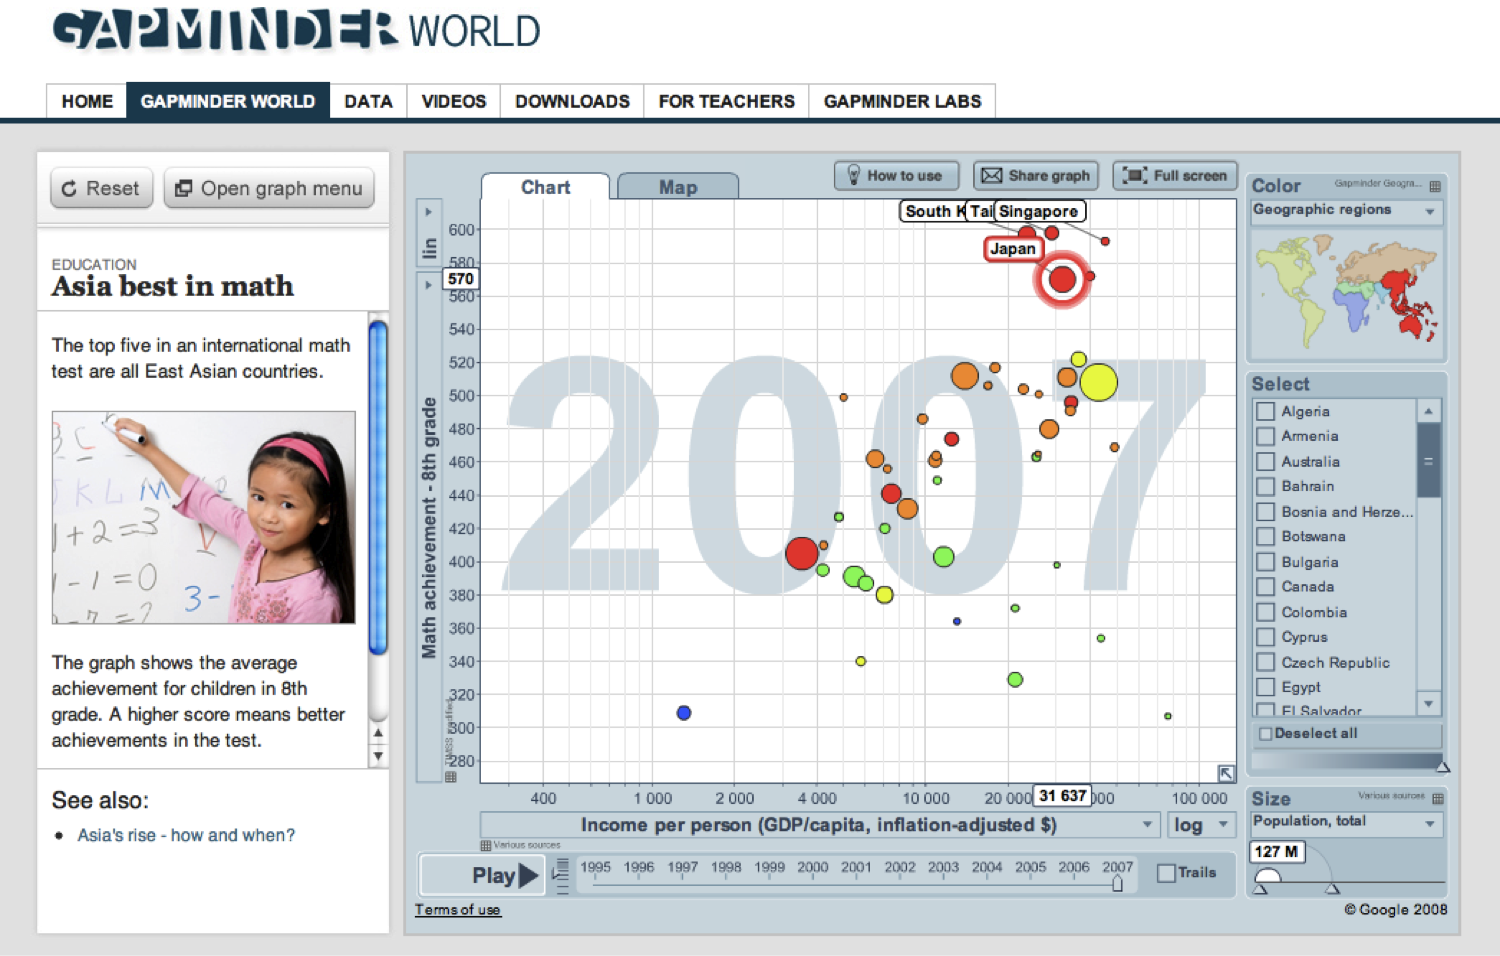
\includegraphics[width=.9\textwidth]{gapminder}}\\[1em]

			\small{See also: ``\href{http://www.ted.com/talks/hans_rosling_shows_the_best_stats_you_ve_ever_seen.html}{Hans Rosling: Stats that reshape your worldview}'' (TED, 2006)}
		\end{center}
		
	\end{frame}
	%
	%

  %
  %
  \subsection{Data portals}
  %
  %

	\begin{frame}[c, plain]

		\begin{center}
			\href{http://www.cessda.org/}%
  			{
\includegraphics[width=.9\textwidth]{data-cessda}}\\[.5em]
			\href{http://www.icpsr.umich.edu/}%
  			{
\includegraphics[width=.9\textwidth]{data-icpsr}}\\[.5em]
			\href{http://www.nsd.uib.no/macrodataguide/}%
  			{
\includegraphics[width=.9\textwidth]{data-nsd}}\\[.5em]
			\href{http://www.data.gov/}%
  			{
\includegraphics[width=.3\textwidth]{data-usgov}}~~%
			\href{http://www.data.gov.uk/}%
  			{
\includegraphics[width=.3\textwidth]{data-ukgov}}~~%
			\href{http://www.data.gouv.fr/}%
  			{
\includegraphics[width=.3\textwidth]{data-frgov}}\\[.5em]
			\href{http://ckan.org//}%
  			{
\includegraphics[width=.9\textwidth]{data-ckan}}\\[1em]
				
			\small{\url{https://github.com/briatte/srqm/wiki/data}}
		\end{center}
		
	\end{frame}
	%
	%
	
	%
	%
	\section{Data structure}
	%
	%

  %
  %
  \subsection{Datasets}
  %
  %
  
	\begin{frame}[t]{Data structures}

	\begin{block}{Cross-sectional data}

		\begin{itemize}
			\item \textbf{Comparable units} sampled over a \red{single time period}
			\item \textbf{Units} can be individual respondents, countries, firms, …
			\item \textbf{Observations} vary by their characteristics, \textit{not} by unit type
		\end{itemize}

  \end{block}

	\begin{block}{Time series}

		\begin{itemize}
			\item \textbf{Repeated observations} over time, pooled or sampled
			\item \textbf{Cross-sectional time series} (CSTS): fixed, nonsampled units
			\item \textbf{Longitudinal data}: e.g. cohorts of patients, stocks, voters, …
		\end{itemize}

  \end{block}

	\end{frame}
  %
  %

  %
  %
  \subsection{Samples}
  %
  %
	
	\begin{frame}[t]{Sample characteristics}

	\begin{block}{Survey methodology}

		\begin{itemize}
			\item Target and survey population
			\item Sampling frame and \textbf{randomization}
			\item Standardized questionnaires
		\end{itemize}
    
  \end{block}

	\begin{alertblock}{Issues in representativeness}

		\begin{itemize}
			\item Undercoverage
			\item Unit nonresponse
			\item Postsurvey adjustments (\textbf{sampling weights})
		\end{itemize}
    
  \end{alertblock}

	\end{frame}
  %
  %

  %
  %
  \subsection{Codebooks}
  %
  %
	
	\begin{frame}[t]{Documentation: \red{codebooks}}
			
  \begin{block}{Contents}

		\begin{itemize}

			\item \textbf{Definitions:} unit of analysis, questionnaire, measurements…
				
			\item \textbf{Survey design:} sampling strategy, time period, weights…

			\item \textbf{Referencing:} authors, affiliations, bibliographic citation
		\end{itemize}
	  
  \end{block}

	\begin{alertblock}{Important}
		
		Knowing the data in depth is never an option: the data is never %
		better than your knowledge of it. ``Garbage In, Garbage Out.'' 
	
	\end{alertblock}	
	
	\end{frame}
	%
	%
	
	\begin{frame}[t]{Example: \red{Quality of Government}}

		Codebook p.~229:

		\begin{center}
			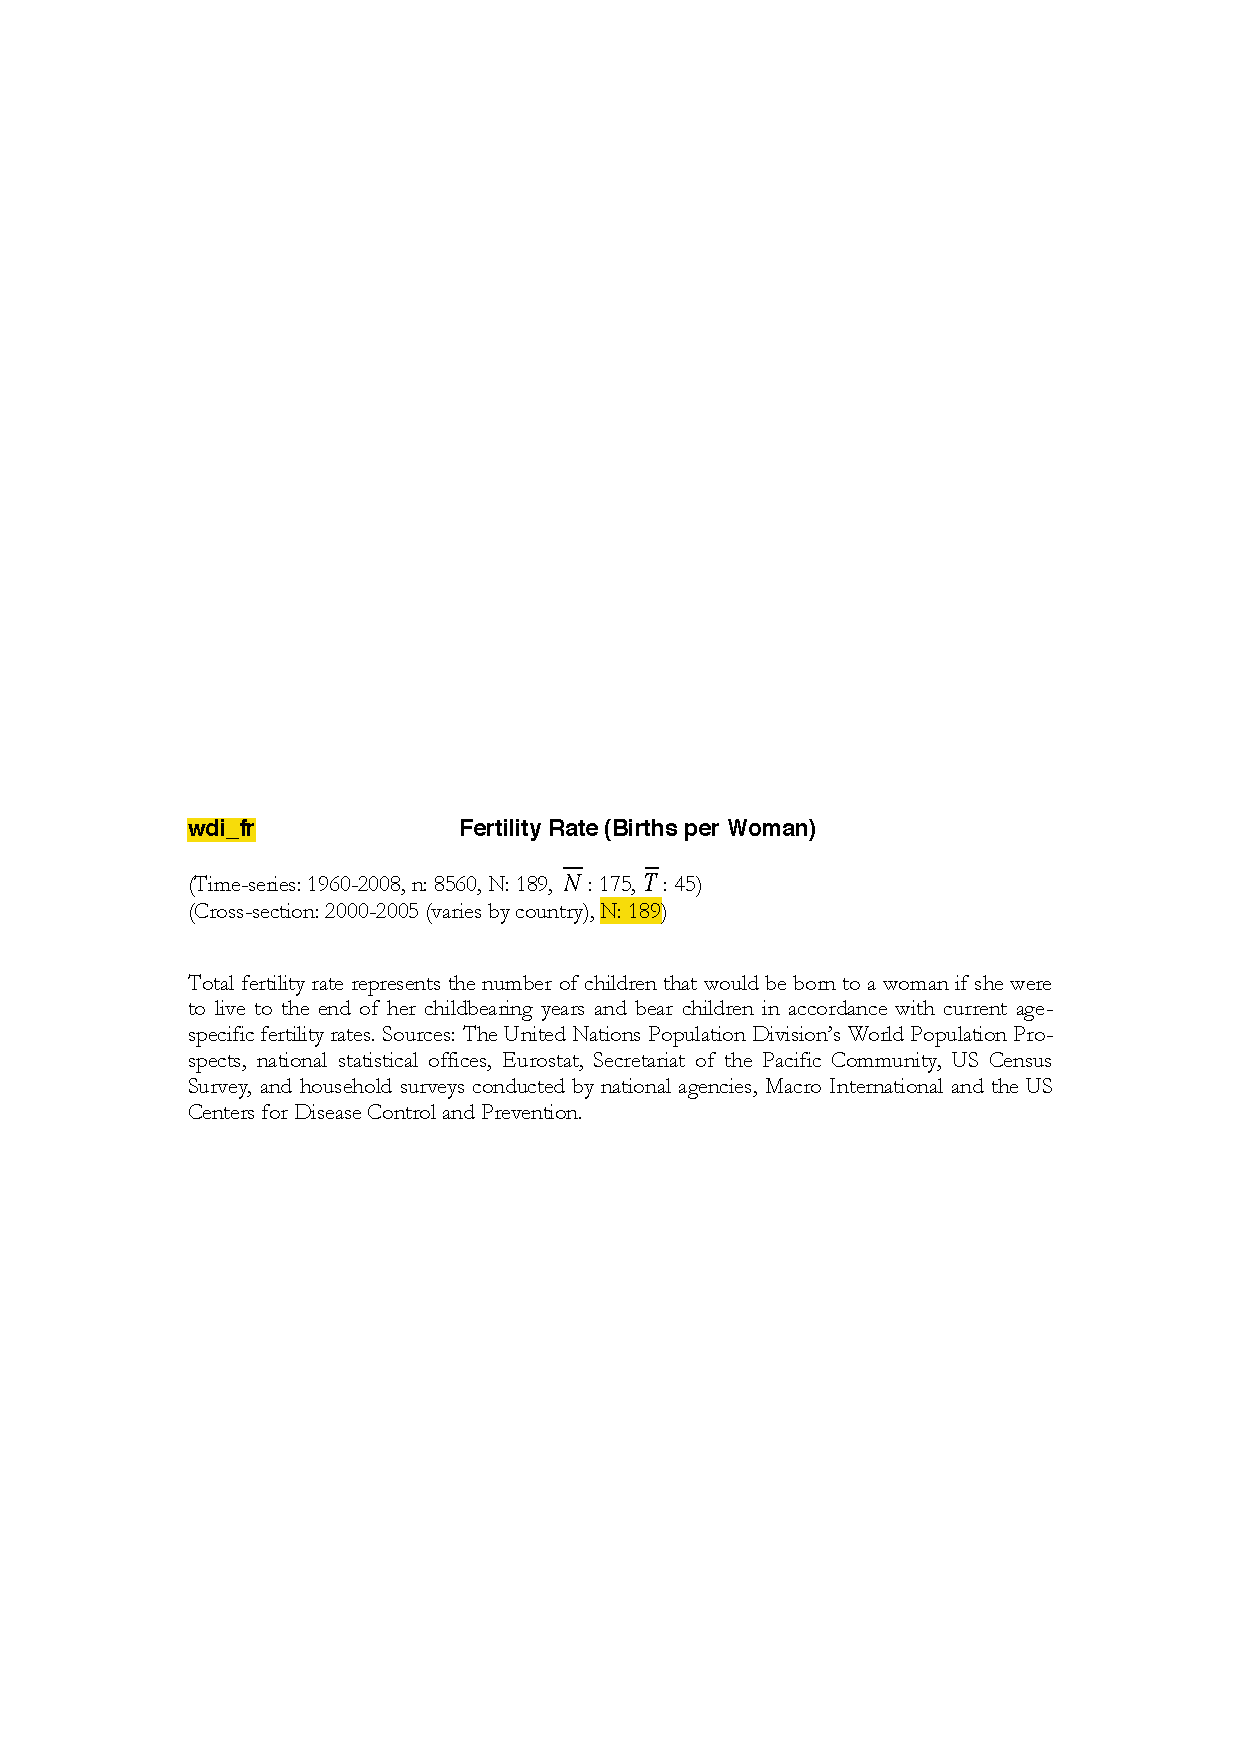
\includegraphics[width=\textwidth]{codebook-qog.pdf}		
		\end{center}
		
	\end{frame}
	%
	%
	
	\begin{frame}[t]{Example: \red{European Social Survey}}
		
    Codebook p.~191:

		\begin{center}
			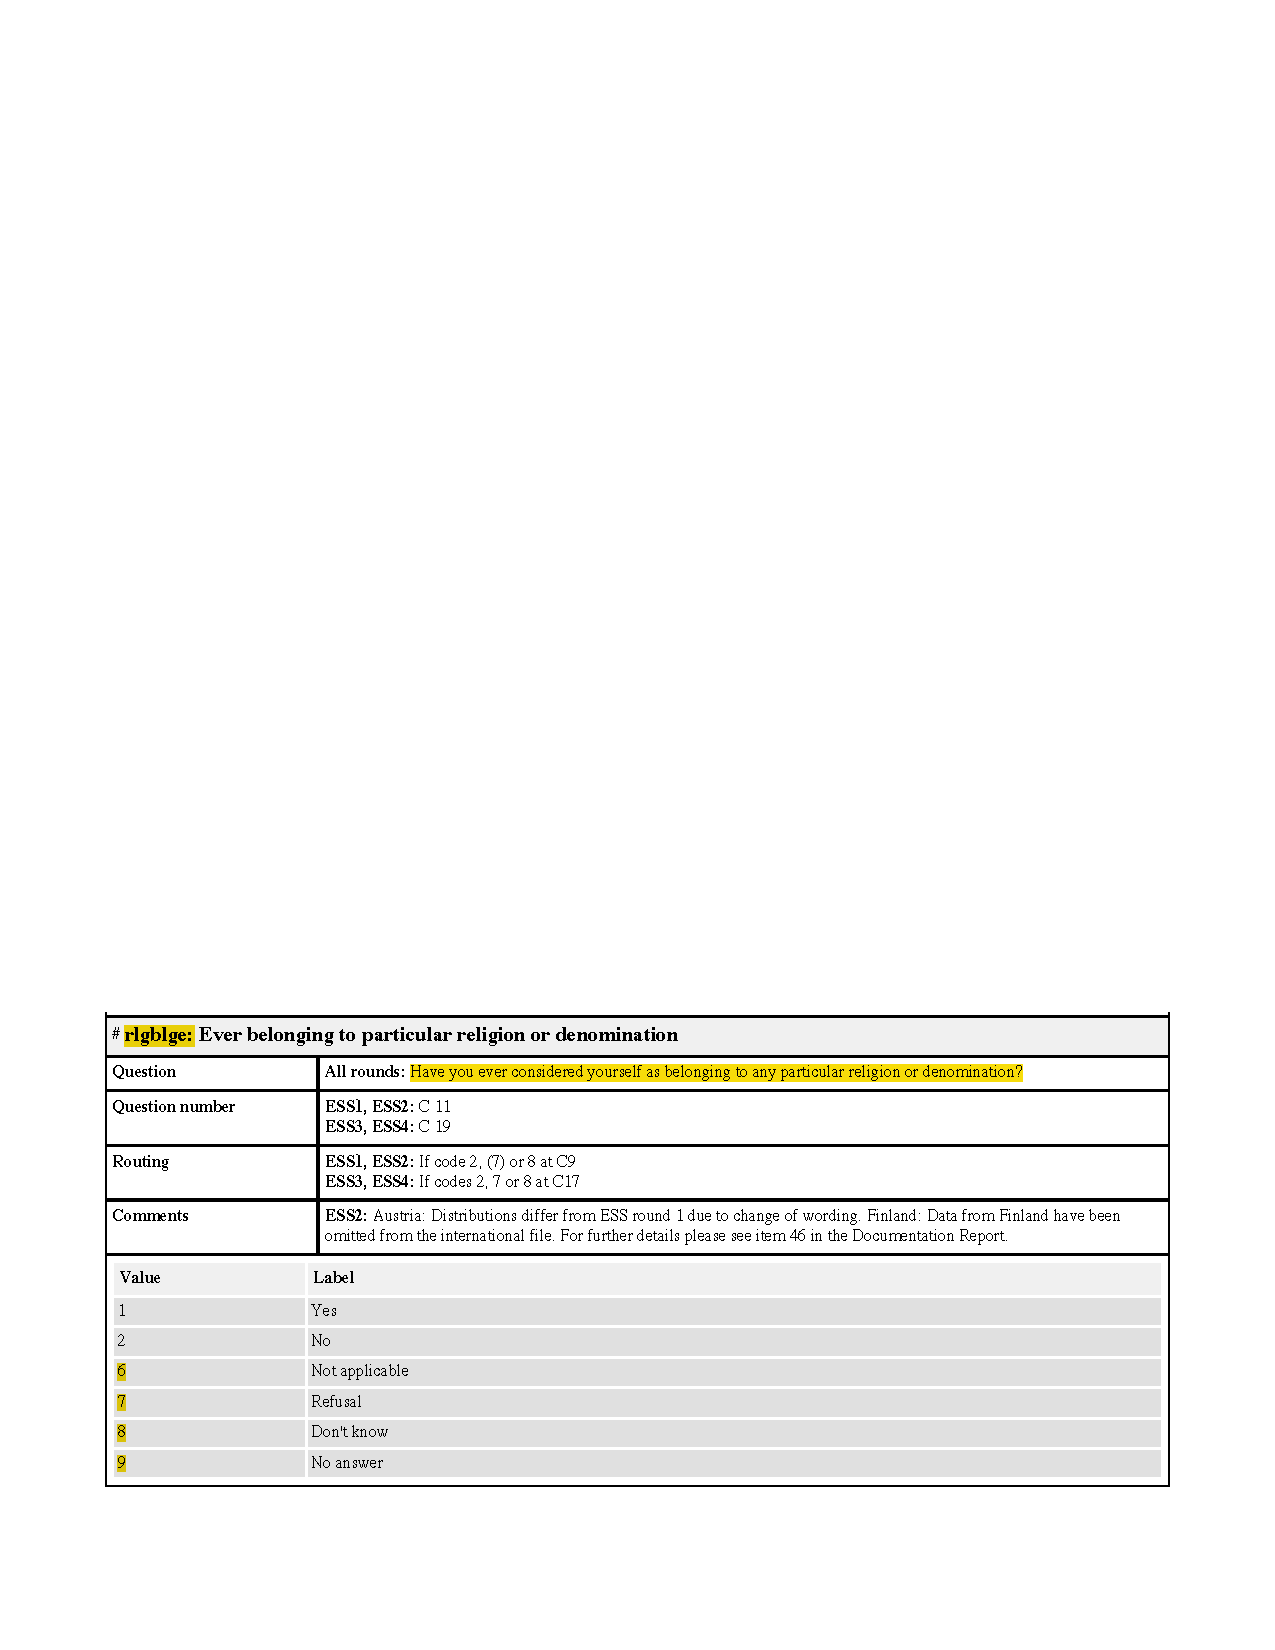
\includegraphics[width=\textwidth]{codebook-ess.pdf}		
		\end{center}

	\end{frame}
  %
  %
	
	%
	%
	\subsection{Formatting}
	%
	%
	
	\begin{frame}[t]{Formatting}
	
	  \begin{block}{Requirements \hfill Stata Guide, Sections 5--8}

			\begin{itemize}
				\item The dataset format is \textbf{DTA} \hfill %
				… otherwise \red{convert}
				
				\item The data is \textbf{cross-sectional} \hfill %
				… otherwise \red{subset}
			
				\item The columns hold \textbf{only variables} \hfill %
				… otherwise \red{reshape}
			\end{itemize}

    \end{block}
		
	  \begin{block}{Course datasets \hfill \texttt{SRQM/data} folder}

			\begin{columns}[T]

				\column{.7\textwidth}

					\begin{itemize}
						\item All files are preprocessed \texttt{.dta}				
						\item \texttt{gss2010} and \texttt{nhis2009} hold several years
						\item See the \texttt{README} file for details
					\end{itemize}
				
				\column{.2\textwidth}
				
					\begin{center}
						\vspace{-1.5em}
						
\includegraphics[width=.8\textwidth]{icon-dta}
					\end{center}
				
			\end{columns}

    \end{block}
		
	\end{frame}
  %
  %
	
	\begin{frame}[t]{Example: \href{http://www.ic.gc.ca/eic/site/ic1.nsf/eng/01464.html}{Industry Canada File Sharing Survey}, 2006}

	Individual-level `micro' data on illegal downloading practices among a random sample of the Canadian population aged 15+:\\[1em]
	
	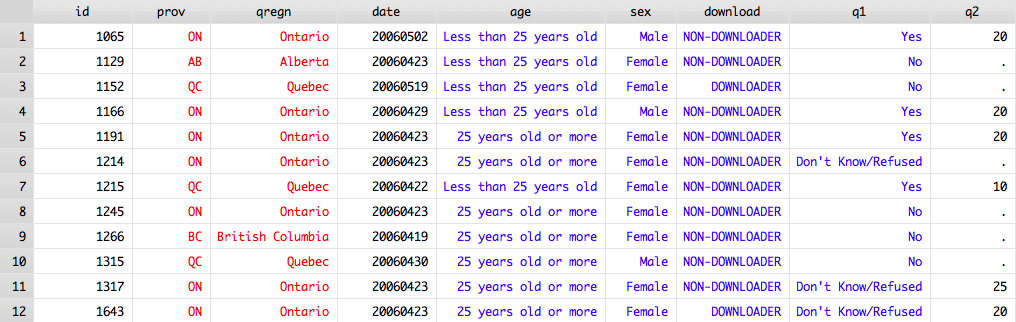
\includegraphics[width=\textwidth]{data-mfss2006}\\[.5em]

  \begin{itemize}
    \item \textbf{Layout:} one observation per row, one variable per column
    \item \textbf{Formats:} \texttt{numeric}, \color{red}{\texttt{string}}, \color{blue}{\texttt{encoded}} \color{fg} (values/labels) 
    \item \textbf{Missing data:} encoded as \texttt{.}~(dot), interpreted as $+\infty$
  \end{itemize}    
 	
	\end{frame}
	%
	%

	%
	%
	\section{Data exploration}
  %
  %
 
	%
	%
	\subsection{Open, describe, search}
	%
	%

	\begin{frame}[t]{Data exploration}
		
	  \begin{block}{Open and describe}
	  	\comm{Load a dataset; -clear- wipes previous data in memory.}\\
		  \code{use data/ess2008, clear}\\
	  
	    \comm{Describe all variables (names and variable labels).}\\
	    \code{describe}\\
	  	    
	    \comm{Describe a few variables (command shorthand:~-d-).}\\
	    \code{d gndr agea edu* trst*}
	  \end{block}
	  
	  \begin{block}{Search for variables}
			\comm{Look for keywords in variable names and labels.}\\
	  	\code{lookfor democ health}\\
	  		  
	  	\comm{The -lookfor\_all- package searches across datasets.}\\
	  	\code{lookfor\_all democ health, dir(data)}
	  \end{block}
	  
	\end{frame}
  %
  %
  		
	%
  %
	\subsection{Selection by range}
	%
	%
	
	\begin{frame}[t]{Selection by \red{range}}
	
		\begin{block}{Browsing and counting}
			
			\comm{All observations have a row number \_n from 1 to \_N.}\\
			\code{di \_N}

	    \comm{List first ten observations.}\\			
			\code{li in 1/10 }\\

			\comm{View entire dataset; NEVER modify the data by hand.}\\
			\code{browse}
		
			\comm{Establish sample size `N'.}\\
			\code{count}
			
		\end{block}

    \begin{exampleblock}{Reminder}
			
      Use \code{help} when you need more details on a command.
    
		\end{exampleblock}
			
	\end{frame}
  %
  %

	%
  %
	\subsection{Selection by conditions}
	%
	%
	
	\begin{frame}[t]{Selection by \red{conditions}}
	
		\begin{block}{Logical operators}

      \comm{Count French and German respondents aged 18 to 24.}\\
      \code{count if (agea >= 18 \& agea < 24) \& ///\\
			~~(cntry == "FR" | cntry == "DE")}

      \comm{Keep observations for a selection of countries.}\\
	    \code{keep if inlist(cntry, "FR", "DE", "IT", "SP")}
				
		\end{block}

	  \begin{block}{Missing values}

	    \comm{Delete data if \underline{mi}ssing age, sex or marital status.}\\
	    \code{drop if mi(agea, gndr, maritala)}\\
	    
	    \comm{Create a married `dummy' variable when applicable.}\\
	    \code{gen married = (maritala == 1) if !mi(maritala)}
	  \end{block}

	\end{frame}
	%
	%

	%
	%
	\subsection{Weights, subsets}
	%
	%
  	
	\begin{frame}[t]{Data preparation}

	  \begin{block}{1. Weight and subset}
		  \comm{Set up survey weights.}\\
		  \code{svyset [pw=dweight]}\\

		  \comm{Keep only some observations.}\\
		  \code{keep if cntry == "FR"}
		\end{block}

	  \begin{block}{2. Subset and count}
	    \comm{Study the missing values for a set of variables.}\\
	    \code{misstable pat gndr agea edulvla trstep}		
			
		  \comm{Drop observations with missing data.}\\
		  \code{drop if mi(gndr, agea, edulvla, trstep)}\\

	    \comm{Get final sample size.}\\
	    \code{count}
		\end{block}

	\end{frame}
  %
  %
	
	%
	%
	\section{Practice}
	%	
	%
	
	%
	%
	\subsection{Example: NHIS dataset}
	%
	%
	
	\begin{frame}[t]{Practice: \red{NHIS dataset}}

		$$\mathsf{Body~Mass~Index} = \frac{\mbox{mass} \ \mbox{(kg)}}{\left( \mbox{height}(\mathsf{m})\right)^2} = \frac{\mbox{mass} \ \mathsf{(lb)} \times 703}{\left(\mbox{height} (\mathsf{in})\right)^2}$$
		
		\vspace{1em}

		\begin{itemize}
			\item For \textbf{normal weight} adults, $18.5 < \mathsf{BMI} < 25$.
			\item For \textbf{overweight} adults, $25 \leq \mathsf{BMI} < 30$.
			\item For \textbf{obese }adults, $\mathsf{BMI} \geq 30$.		
		\end{itemize}

		\vspace{1em}
		
    Data:
	
			\begin{columns}[c]
				\column{.725\textwidth}
				
				\begin{itemize}
					\item National Health Interview Survey (NHIS)
					\item Sample: U.S. adult population, 2009
				\end{itemize}
	
				\column{.2\textwidth}
				
\includegraphics[width=\textwidth]{logo-nhis}
			\end{columns}
	
	\end{frame}
	%
	%

  %
  %
	\subsection{Maps}
	%
	%
	
  \begin{frame}[t, plain]{}
	  \absoluteimage{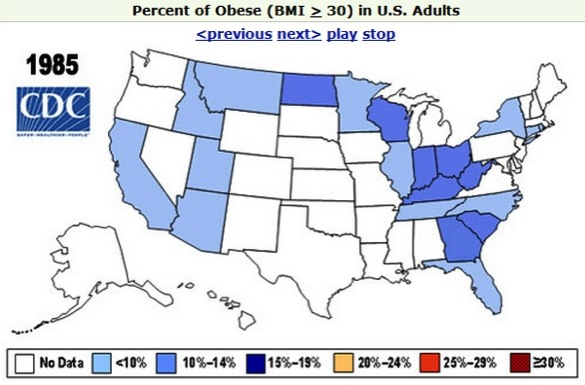
\includegraphics[width=\paperwidth]{map-cdc-1}}
  \end{frame}

  \begin{frame}[c, plain]{}
	  \absoluteimage{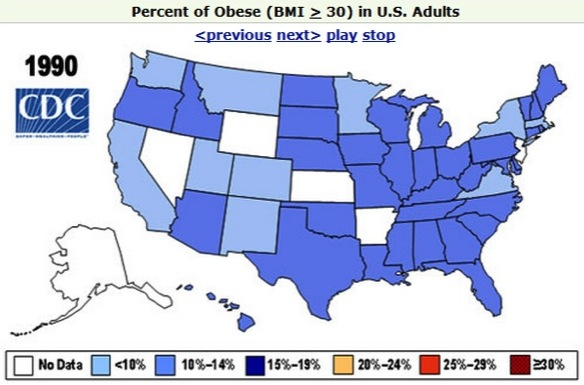
\includegraphics[width=\paperwidth]{map-cdc-2}}
  \end{frame}

  \begin{frame}[c, plain]{}
	  \absoluteimage{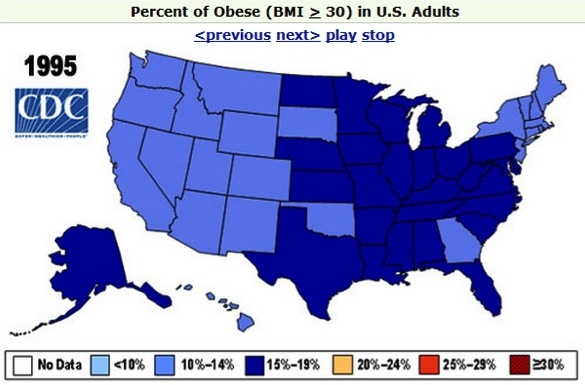
\includegraphics[width=\paperwidth]{map-cdc-3}}
  \end{frame}

  \begin{frame}[c, plain]{}
	  \absoluteimage{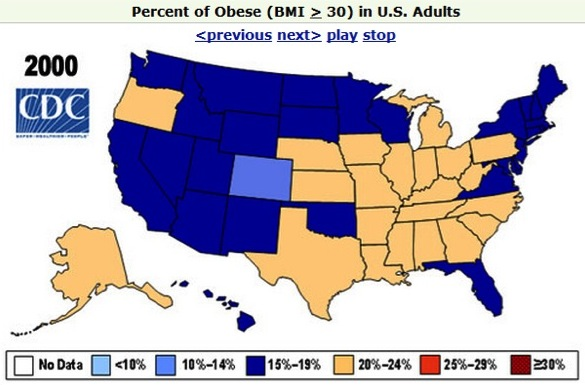
\includegraphics[width=\paperwidth]{map-cdc-4}}
  \end{frame}

  \begin{frame}[c, plain]{}
	  \absoluteimage{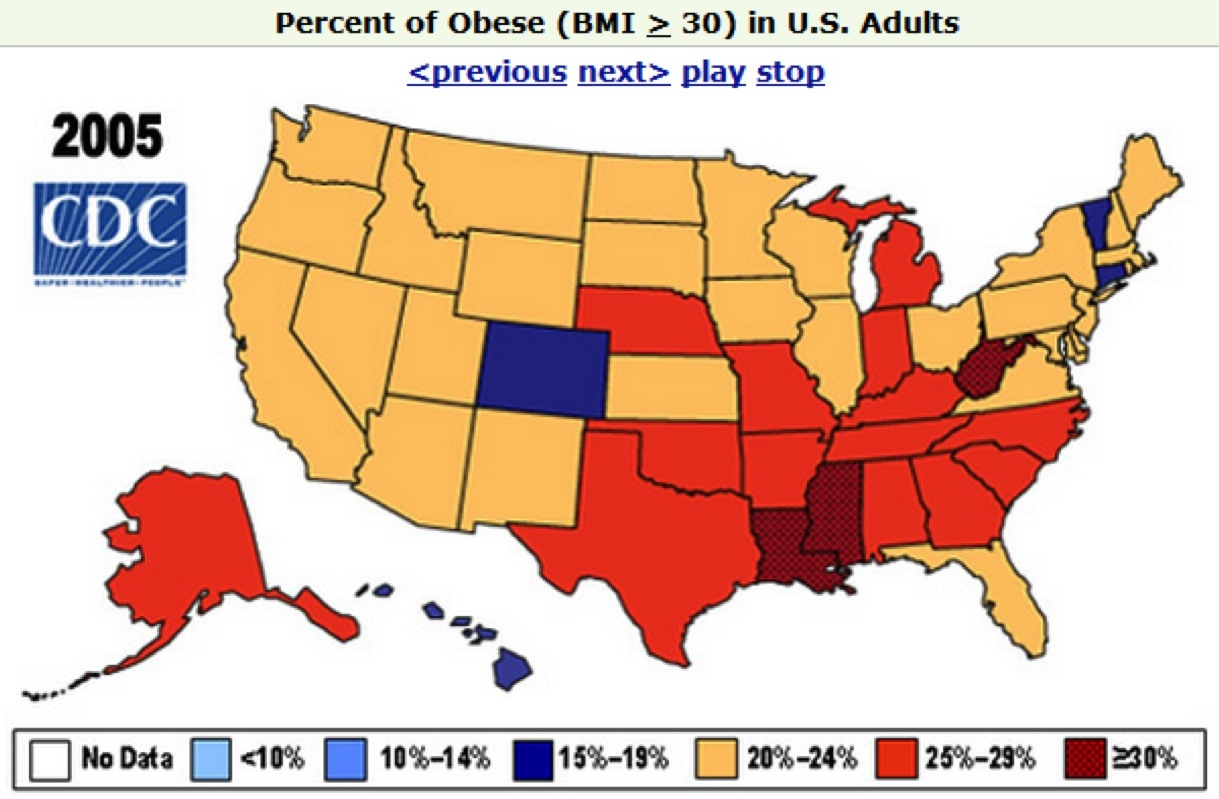
\includegraphics[width=\paperwidth]{map-cdc-5}}
  \end{frame}

  \begin{frame}[c, plain]{}
	  \absoluteimage{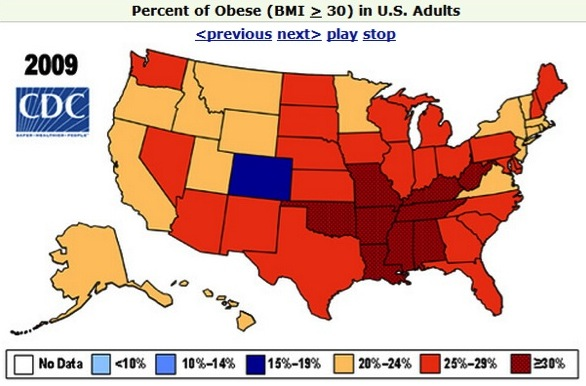
\includegraphics[width=\paperwidth]{map-cdc-6}}
  \end{frame}

  \begin{frame}[c, plain]{Another dimension of the issue}
	  \absoluteimage{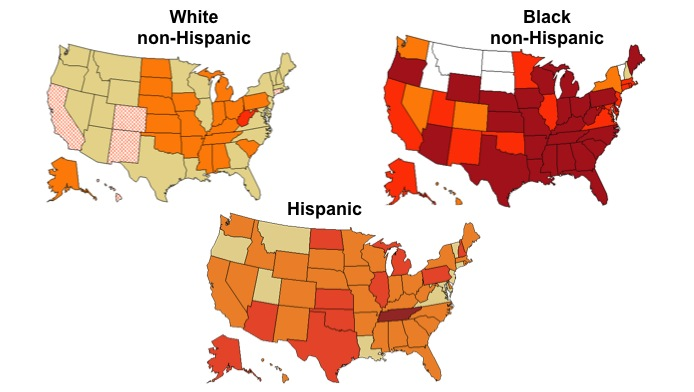
\includegraphics[width=\paperwidth]{map-cdc-7}}
  \end{frame}
	
	%
	%
	\subsection{Coursework}
  %
  %
  
	\begin{frame}[t]{Practice session}

    \begin{block}{Class}
      \comm{Get the do-file for this week.}\\
      \code{srqm fetch week2.do}\\
      
			\comm{Open to read and replicate.}\\
			\code{doedit code/week2}\\    
    \end{block}

    \begin{alertblock}{Coursework}
      \begin{itemize}
	       \item Finish the do-file and read all comments at home.
	       \item Read from the codebooks in the \texttt{data/} folder. 
	       \item Start writing some draft code to describe a dataset.
      \end{itemize}
    \end{alertblock}
    		
	\end{frame}
  %
  %
  
  %
  %
  \subsection{Exercises}
  %
  %
  
  \begin{frame}{Exercises}

    \begin{exampleblock}{Ex~2.1. European Social Survey 2008}
      \begin{enumerate}
        \item Load the data.
        \item Find all variables on discrimination.
        \item How many countries are there in the dataset?
      \end{enumerate}
    \end{exampleblock}
		
    \begin{exampleblock}{Ex.~2.2. Quality of Government 2011}
      \begin{enumerate}
        \item Load the data.
        \item Find all variables on corruption.
        \item Which one has the most observations?
      \end{enumerate}
    \end{exampleblock}

  \end{frame}
  %
  %  
	
\end{document}